% Neural-ODE decoder in radius.  Build: latexmk -pdf node.tex
\documentclass[border=8pt]{standalone}
\usepackage{amsmath}
% Shared TikZ palette + node styles for the ML-RT2 architecture diagrams.
% Colours match the ML-RT comparison-paper figures so the three papers look consistent:
%   pink   = data / vectors (inputs, outputs, latent representations)
%   blue   = learned networks / operators (MLPs, encoders, decoders, ...)
%   orange = special operations / physics (spectral transforms, RT residual, ...)
%   green  = loss / training terms
\usepackage{tikz}
\usetikzlibrary{arrows.meta,positioning,fit,backgrounds,calc}

\definecolor{dataFill}{HTML}{F2E6FF}\definecolor{dataDraw}{HTML}{6600CC}
\definecolor{netFill}{HTML}{B5E8E8}\definecolor{netDraw}{HTML}{086565}
\definecolor{opFill}{HTML}{FFE0C2}\definecolor{opDraw}{HTML}{AB4F03}
\definecolor{lossFill}{HTML}{C8F4C1}\definecolor{lossDraw}{HTML}{0C5600}

\tikzset{
  font=\small,
  box/.style  ={draw, rounded corners, align=center, inner sep=4pt, minimum height=9mm, line width=0.3mm},
  data/.style ={box, fill=dataFill, draw=dataDraw},
  net/.style  ={box, fill=netFill,  draw=netDraw},
  op/.style   ={box, fill=opFill,   draw=opDraw},
  loss/.style ={box, fill=lossFill, draw=lossDraw},
  sum/.style  ={draw=netDraw, circle, inner sep=1.3pt, fill=white, line width=0.3mm},
  arr/.style  ={-{Stealth[length=2.4mm]}, thick},
  darr/.style ={-{Stealth[length=2.4mm]}, thick, dashed},
  note/.style ={align=center, font=\scriptsize, text=black!65},
}

\begin{document}
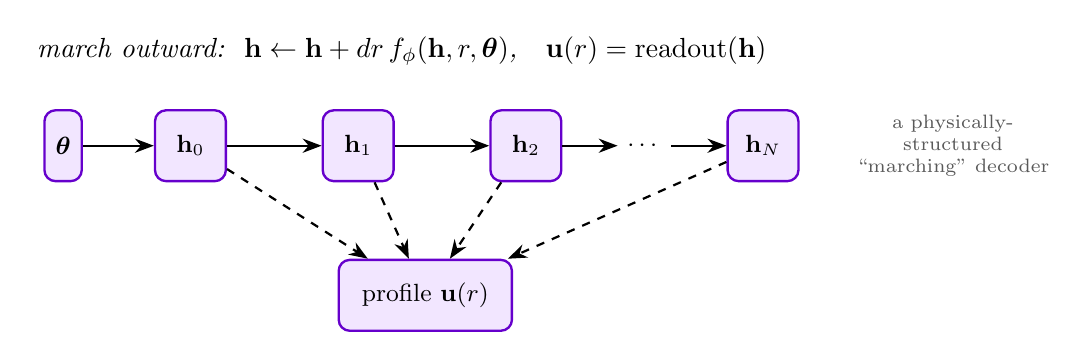
\begin{tikzpicture}
  % update rule as a single caption above the chain (not on every arrow)
  \node[font=\itshape] (rule) at (4.3,1.2)
        {march outward:\ \ $\mathbf{h}\leftarrow \mathbf{h}+dr\,f_\phi(\mathbf{h},r,\boldsymbol{\theta})$,\quad
         $\mathbf{u}(r)=\mathrm{readout}(\mathbf{h})$};

  \node[data] (th) at (0,0)                 {$\boldsymbol{\theta}$};
  \node[data, minimum width=9mm, right=9mm of th]  (h0) {$\mathbf{h}_0$};
  \node[data, minimum width=9mm, right=12mm of h0] (h1) {$\mathbf{h}_1$};
  \node[data, minimum width=9mm, right=12mm of h1] (h2) {$\mathbf{h}_2$};
  \node[right=7mm of h2]                     (hd) {$\cdots$};
  \node[data, minimum width=9mm, right=7mm of hd]  (hn) {$\mathbf{h}_N$};
  \foreach \a/\b in {th/h0, h0/h1, h1/h2, h2/hd, hd/hn} \draw[arr] (\a) -- (\b);

  % readouts to the profile
  \node[data, minimum width=22mm] (out) at (4.6,-1.9) {profile $\mathbf{u}(r)$};
  \foreach \n in {h0,h1,h2,hn} \draw[darr] (\n) -- (out);
  \node[note, right=6mm of hn] {a physically-\\structured\\``marching'' decoder};
\end{tikzpicture}
\end{document}
